\documentclass[conference]{IEEEtran}
\IEEEoverridecommandlockouts
\usepackage{cite}
\usepackage{amsmath,amssymb,amsfonts}
\usepackage{algorithm}
\usepackage{algorithmic}
\usepackage{graphicx}
\usepackage{textcomp}
\usepackage{xcolor}
\usepackage{booktabs}
\usepackage{url}
\begin{document}

\title{A Controlled Comparison of Causal Scoring Rules for Root Cause Analysis in Spine-Leaf Datacenter Networks}


\author{
\IEEEauthorblockN{Navin Suvarna*}
\IEEEauthorblockA{Independent Researcher\\
Holly Springs, NC, USA\\
nsuvarna@cisco.com\\
0009-0004-0161-2372}
*Corresponding author
\and
\IEEEauthorblockN{Karthik Pappu}
\IEEEauthorblockA{Dakota State University\\
Madison, SD, USA\\
karthik.pappu@trojans.dsu.edu\\
0009-0000-5335-6279}
\and
\IEEEauthorblockN{Saurabh Sharma}
\IEEEauthorblockA{Independent Researcher\\
Apex, NC, USA\\
saurabh.sharma24@gmail.com\\
0009-0001-5486-8062}
\and
\IEEEauthorblockN{Ankit Parashar}
\IEEEauthorblockA{Independent Researcher\\
Indianapolis, IN, USA\\
ankitparashar.ec.2110@gmail.com\\
0009-0008-6656-450X}
}

\maketitle

\begin{abstract}
Causal root cause analysis for datacenter fabrics rests on two design choices: where the dependency graph comes from, and how candidates are scored over it. Published systems vary both at once, so it is unclear which one does the work. We hold the graph fixed and vary only the scoring rule, using one architecture-derived graph over 28 spine-leaf metrics, healthy-only training and one protocol throughout, and compare four rules: counterfactual restoration, residual scoring in the style of CIRCA, distributional divergence in the style of MicroCause, and anomaly magnitude. We also correct a defect in intervention scoring as it is usually formulated, which discards the evidence on the candidate itself; the correction is worth five points of Top-1 accuracy and is what makes the comparison fair. Over 860 incidents from 20 seeds, residual scoring is the most accurate rule at 0.664 Top-1, ahead of counterfactual restoration at 0.547 and anomaly magnitude at 0.405, with every pairwise difference significant. The gap arises on incidents where the root is already the most anomalous metric, because the counterfactual rule's downstream term is large enough to override a signal that was already right. Two findings about evaluation matter as much: restricting candidates to the metrics where faults were injected makes all four rules indistinguishable, and an effect measured at five seeds shrinks fivefold at forty. Structure discovery on real telemetry recovers one edge across forty metrics, so on that corpus the graph had to come from the architecture.
\end{abstract}

\begin{IEEEkeywords}
root cause analysis, causal inference, datacenter networks, structural equation modeling, counterfactual reasoning, benchmark design
\end{IEEEkeywords}

\section{Introduction}
Modern datacenter networks operate under demanding availability targets, and even short disruptions can reach end users. Spine-leaf fabrics are widely deployed because they offer high bisection bandwidth and path redundancy at scale \cite{alfares2008fattree,greenberg2009vl2}. The same layering that delivers that performance also couples failures together. Physical optics, link utilization, queueing, a distributed control plane such as the Border Gateway Protocol (BGP) \cite{rekhter2006bgp}, and an overlay such as Virtual eXtensible LAN (VXLAN) \cite{mahalingam2014vxlan} all interact. One initiating fault can raise alarms on a dozen metrics at once, and the metric that looks worst is frequently a consequence rather than the cause.

Causal approaches to root cause analysis (RCA) attack this directly, representing directed dependencies among metrics and using them to separate causes from effects \cite{pearl2009causality,peters2017elements}. Every such system makes two independent choices. The first is where the dependency graph comes from, whether learned from data or supplied by domain knowledge. The second is how a candidate is scored once the graph exists, whether by a counterfactual intervention, a regression residual, or a distributional shift. Published systems differ in both choices at once, and are evaluated on different datasets with different metrics, so the literature offers little guidance on which choice matters.

This paper isolates the second choice. We fix the graph, the training data, the candidate set, and the protocol, and vary only the scoring rule. That makes the comparison controlled, and it lets us settle a question the field has left open: whether a more elaborate scoring rule ranks better once the dependency graph is already correct.

The answer turned out to depend on how the benchmark is constructed, which became the more useful contribution. Three questions organize the work.
\label{sec:rqs}
\textbf{RQ1:} Among scoring rules over a shared architecture-derived causal graph, which identifies root causes most accurately, and why?
\textbf{RQ2:} How much do the definition of the candidate set and the size of the evaluation change that answer?
\textbf{RQ3:} Can the required causal structure be recovered from production telemetry, or must it come from the architecture?

This paper makes four contributions. First, a comparison of four scoring rules over one graph, one training regime and one protocol, on 860 incidents from 20 seeds, with a paired significance test for every claim; residual scoring wins. Second, an explanation of why: the counterfactual term is roughly five times larger relative to a candidate's own deviation than the residual term is, so it overrides the anomaly ordering far more often, including where that ordering was already correct, and it is not ahead in any of the five regimes we examined, four of them specified before testing. Third, two findings about benchmarking: restricting the candidate set to known fault locations makes all four rules statistically indistinguishable and lets a graph-free baseline match the full pipeline exactly, and an effect measured at five seeds shrinks fivefold and loses significance at forty. We took both shortcuts ourselves before measuring what they cost. Fourth, a correction to intervention scoring itself, whose standard formulation discards the evidence on the candidate and, left uncorrected, would have confounded the comparison. We also show that data-driven structure discovery on real telemetry recovers a near-empty graph.

The remainder of this paper is organized as follows. Section~\ref{sec:related} reviews prior work on fault localization and causal RCA. Section~\ref{sec:model} defines the fabric model, the candidate set, and the ranking problem. Section~\ref{sec:method} specifies the four scoring rules. Section~\ref{sec:eval-setup} describes the data, its calibration against published failure measurements, and the evaluation protocol. Section~\ref{sec:results} reports the comparison, and Section~\ref{sec:discussion} discusses implications and limitations.

\section{Related Work}
\label{sec:related}
Early datacenter fault-diagnosis systems built dependency graphs from measurement and ran probabilistic inference over them. Sherlock \cite{bahl2007sherlock} infers a multi-level dependency graph from packet traces and localizes faults by likelihood, while NetPoirot \cite{arzani2016netpoirot} trains a classifier on endpoint TCP features. Gestalt \cite{mysore2014gestalt} unifies several such inference algorithms, and large-scale measurement work characterizes what actually breaks \cite{kandula2009detailed,gill2011understanding}. These systems established that dependency structure is essential for localization. They share one limit: their graphs come from traffic co-occurrence or active probing, so an edge records observed association rather than a mechanism. Such a graph cannot answer the question an operator asks, which is whether fixing a component would remove the symptoms.

A second line brings explicit causal machinery to service telemetry. CauseInfer \cite{chen2014causeinfer} builds a two-layer causality graph and walks it. MicroCause \cite{meng2020microcause} ranks metrics by distributional divergence with a path-aware traversal, REASON \cite{wang2023reason} models hierarchical networks, and CORAL \cite{wang2023coral} updates structure online. CIRCA \cite{li2022circa} is closest to our setting: it treats an incident as an intervention, fits regressions on healthy data, and scores each candidate by the residual between its observed value and the value predicted from its parents.

What none of this work does is separate the graph from the scoring rule. CIRCA and MicroCause differ in their graphs, datasets, candidate sets and metrics as well as in how they score, so a reader cannot tell whether CIRCA's advantage comes from residual scoring or from a better graph. Our contribution is to remove every difference except the scoring rule. A second gap concerns evaluation rather than method. An earlier version of this work ranked candidates drawn only from the metrics where faults had been injected, and reported on a few hundred incidents from five seeds. Section~\ref{sec:results-candset} shows that either choice can reverse the conclusion, which is why we report both settings here rather than only the one that flatters our own rule. Table~\ref{tab:relatedwork} summarizes the positioning. In it, \emph{Counterfactual} means explicit $\mathrm{do}(\cdot)$ semantics, with \emph{partial} denoting a residual-based proxy; \emph{Controlled} means the scoring rule is isolated with graph, data and protocol held fixed; and \emph{Healthy-only} means the structural model is trained without incident data.

\begin{table}[htbp]
\caption{Positioning relative to prior RCA work.}
\label{tab:relatedwork}
\centering
\resizebox{\columnwidth}{!}{%
\begin{tabular}{lccccc}
\toprule
\textbf{Work} & \textbf{Net RCA} & \textbf{Counterfact.} & \textbf{Graph Source} & \textbf{Controlled} & \textbf{Healthy-only} \\
\midrule
Sherlock \cite{bahl2007sherlock}              & \checkmark & --         & Heuristics/probing      & -- & -- \\
NetPoirot \cite{arzani2016netpoirot}          & \checkmark & --         & Learned deps.           & -- & -- \\
MicroCause \cite{meng2020microcause}          & --         & --         & Data-driven             & -- & -- \\
CIRCA \cite{li2022circa}                      & --         & partial    & Domain/learned          & -- & \checkmark \\
REASON \cite{wang2023reason}                  & --         & --         & Data-driven             & -- & -- \\
CORAL \cite{wang2023coral}                    & --         & --         & Online discovery        & -- & -- \\
\textbf{This paper}                           & \checkmark & \checkmark & Architecture-derived    & \checkmark & \checkmark \\
\bottomrule
\end{tabular}%
}
\end{table}

\section{System Model and Problem Formulation}
\label{sec:model}

\subsection{Spine-Leaf Fabric and Telemetry}
We consider a spine-leaf fabric of spine switches, top-of-rack (ToR) leaf switches, and attached servers, shown in Fig.~\ref{fig:architecture}. The topology follows a folded-Clos design with redundant leaf-to-spine links and multiple equal-cost paths for east-west traffic \cite{alfares2008fattree,greenberg2009vl2}. An overlay provides logical segmentation \cite{mahalingam2014vxlan}, and BGP maintains reachability and policy \cite{rekhter2006bgp}.

\begin{figure}[htbp]
\centering
\resizebox{0.78\columnwidth}{!}{%
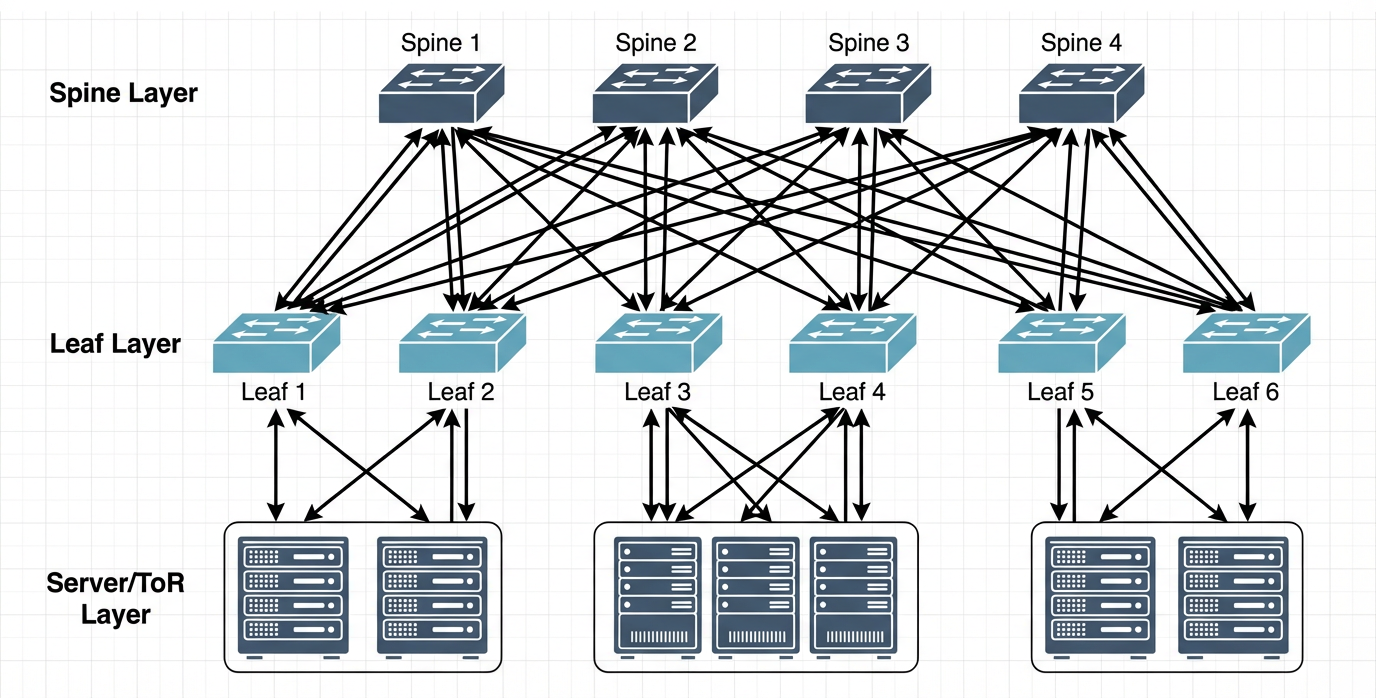
\includegraphics{figure1-architecture-v1.png}%
}
\caption{Spine-leaf fabric: a two-stage folded-Clos topology \cite{alfares2008fattree,greenberg2009vl2} with redundant spine-to-leaf connectivity and dual server attachment.}
\label{fig:architecture}
\end{figure}

Telemetry is sampled every 10\,s and spans four layers: a physical layer (optical receive power, bit error rate, link utilization, packet loss), a control-plane layer (BGP update rate, route flaps, convergence indicators, routing-loop signals), an overlay layer (VXLAN tunnel endpoint reachability, encapsulation and decapsulation errors), and a server-facing layer (CPU utilization, retransmissions, application latency, connection timeouts).

Let $\mathbf{X}_t=(X_1^t,\ldots,X_m^t)$ be the metric vector at time $t$. Directed dependencies are represented by a directed acyclic graph (DAG) $\mathcal{G}=(\mathcal{V},\mathcal{E})$ in which a node is a metric and an edge $(u\!\to\!v)$ encodes an assumed causal influence \cite{pearl2009causality,peters2017elements}. For a node $j$ we write $\mathrm{pa}(j)$ for its set of parents and $\mathrm{Desc}(j)$ for the set of its descendants, meaning every node reachable from $j$ along directed edges. For the fabric modelled here, $|\mathcal{V}|=28$ and $|\mathcal{E}|=26$, and the longest chain runs five hops from optical degradation to application timeouts.

\subsection{Anomaly Scoring and the Candidate Set}
Per-metric baselines are estimated on healthy telemetry alone. For metric $X_i$ with healthy mean $\mu_i$ and standard deviation $\sigma_i$, the anomaly score is the standardized deviation
\begin{equation}
S_{\mathrm{anom}}(i) \;=\; \left|\frac{X_i^t-\mu_i}{\sigma_i}\right|,
\label{eq:sanom}
\end{equation}
and metric $i$ is flagged at time $t$ when $S_{\mathrm{anom}}(i)\ge\tau$, with $\tau=3$. Writing $\mathcal{A}_t$ for the flagged set, the candidate root set over an incident window $\mathcal{T}$ is
\begin{equation}
\mathcal{C}=\bigcup_{t\in \mathcal{T}} \mathcal{A}_t .
\label{eq:candidate-set}
\end{equation}

Equation~\eqref{eq:candidate-set} deserves emphasis, because Section~\ref{sec:results-candset} shows it decides the paper's main comparison. The candidate set contains every metric that became anomalous, which includes downstream consequences of the fault as well as the fault itself. A ranker must therefore reject a symptom in favor of its own cause. Restricting $\mathcal{C}$ instead to a short list of known fault locations removes exactly that difficulty, and with it much of the need for causal reasoning.

\subsection{Problem Statement}
\label{sec:problem}
\emph{Given} an architecture-derived DAG $\mathcal{G}$ over $m$ metrics; healthy telemetry sufficient to estimate baselines $(\mu_i,\sigma_i)$ and per-edge structural equations $f_{(p,j)}$; and an incident window $\mathcal{T}$ with candidate set $\mathcal{C}$ from \eqref{eq:candidate-set},
\emph{find} an ordering of $\mathcal{C}$
\emph{that maximizes} the probability that the true initiating metric $r^{*}$ appears at the head, subject to a per-incident cost small enough for interactive triage.

Writing $r_1$ for the candidate at the head of the ordering, we measure Top-1 accuracy $\mathrm{Acc}_1=\Pr[r_1=r^{*}]$, where correctness means exact identification of the metric into which the fault was injected. For incidents with two injected roots we report Top-$k$@coverage, the probability that at least one of the two true roots appears among the first $k$ candidates. In every table, $\Delta$ is the paired per-incident difference in accuracy between the two rules named in the column heads.

\section{Scoring Rules Compared}
\label{sec:method}
All rules operate on the same graph, the same healthy-only structural equations, and the same candidate set. They differ only in how a candidate is scored.

\subsection{Shared Components}
The graph is derived from the fabric architecture and held fixed; it is not learned from incident data. Each edge asserts a mechanism documented by a protocol specification, a vendor datasheet, or the Clos topology. As shown in Fig.~\ref{fig:datacenter_dag}, the result has 28 nodes, 26 edges, density 0.034, and depth five. Edges fall into five provenance classes, with counts in parentheses: physical-optical (3, optics specifications and Clos topology \cite{alfares2008fattree}); queue and utilization (9, Clos-fabric queueing \cite{alfares2008fattree,greenberg2009vl2}); loss and retransmission (5, TCP semantics, RFC 5681); control-plane (7, BGP-4 update propagation \cite{rekhter2006bgp}); and overlay (2, VXLAN encapsulation and decapsulation \cite{mahalingam2014vxlan}). Three exclusion rules keep it sparse: no transitive edges whose effect is carried by an intermediate node, no edges skipping a layer of abstraction, and no edges whose healthy-data fit is negligible ($R^2<0.05$).

\begin{figure}[htbp]
\centering
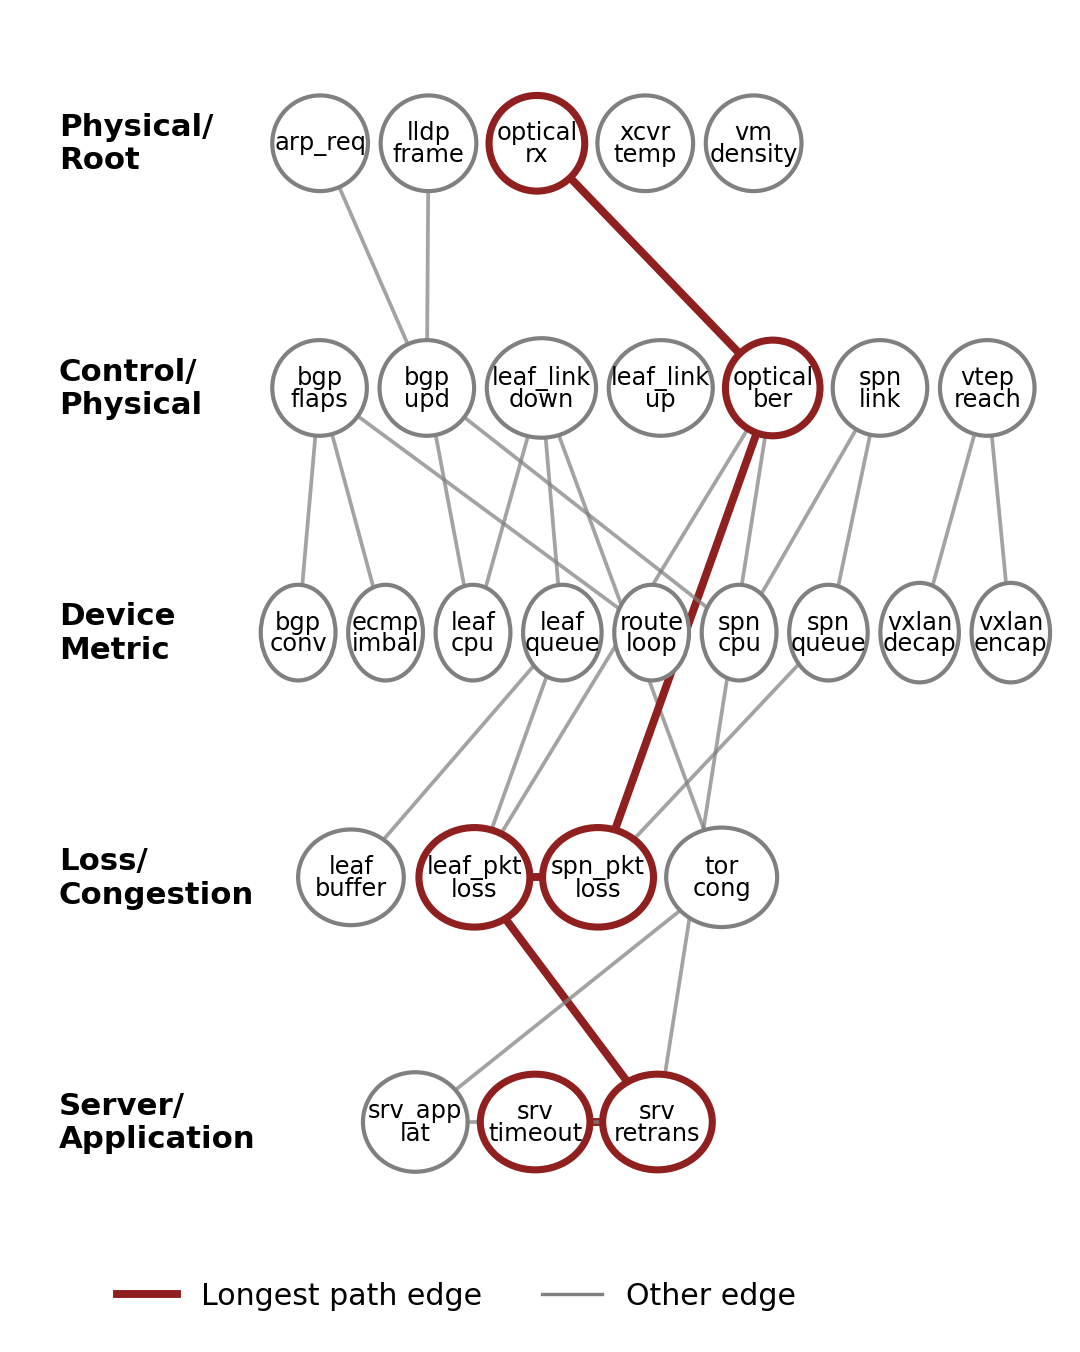
\includegraphics[width=0.88\columnwidth]{figure2_datacenter_dag.png}
\caption{Architecture-derived causal DAG over the 28 spine-leaf metrics (26 edges, density 0.034, longest path five). Nodes are grouped by layer. The bold path traces the longest chain, from optical degradation to server connection timeouts. Node labels are abbreviated: \texttt{optical\_rx} is optical receive power, \texttt{optical\_ber} bit error rate, \texttt{leaf\_link\_down} leaf downlink utilization, \texttt{bgp\_upd} BGP update rate, \texttt{bgp\_flaps} route flaps, \texttt{srv\_retrans} server retransmissions and \texttt{srv\_timeout} connection timeouts.}
\label{fig:datacenter_dag}
\end{figure}

For every edge $(p\!\to\!j)$ in $\mathcal{G}$ we fit a univariate ordinary-least-squares model $f_{(p,j)}$ that predicts $X_j$ from $X_p$ alone, using healthy windows only \cite{pearl2009causality}. A node with several parents therefore carries one model per incoming edge rather than a single multivariate regression over $\mathrm{pa}(X_j)$, and the per-edge estimates are combined at scoring time. The two leading rules combine them differently, so each combination rule is stated with its rule below. Of the 28 metrics, 13 have one parent, 5 have two and 1 has three, so the combination step is inactive for most nodes. Training on incident data would fold fault-induced correlations into the baseline, so the model would treat a symptom as normal.

An audit of edge-wise fit shows a split distribution: twelve edges (46.2\%) reach $R^2>0.5$ and cover the leaf congestion path, the BGP route-flap path, the optical-to-bit-error edge, and the server retransmission path; seven sit between $0.1$ and $0.5$; the remaining seven fall below $0.1$ and lie almost entirely in the spine link-utilization layer and the VXLAN overlay, where the generator drives each metric with largely independent noise. Aggregate fit is mean $R^2=0.467$, median $0.471$. Weak edges are down-weighted rather than pruned, by setting $w_j=\max_{p\in\mathrm{pa}(j)} R^2_{(p,j)}$ and zeroing contributions below $0.05$. Nineteen of the 26 edges survive that filter and carry the ranking.

\subsection{The Four Rules}
\emph{Anomaly magnitude} ranks candidates by $S_{\mathrm{anom}}$ from \eqref{eq:sanom}. It ignores the graph entirely and is the floor any causal method must clear.

\emph{Counterfactual restoration} simulates repairing the candidate. We set $X_r$ to its healthy mean and propagate breadth-first through its descendants using the per-edge models. A descendant reached for the first time takes that edge's estimate; one reached again through a second parent takes the mean of its current value and the new estimate. For the single node with three parents this running mean weights the later-visited parent more heavily, which we note because it is an implementation choice rather than a property of the model. Writing $\hat{X}_j^{\mathrm{do}(r)}$ for the resulting value, $S_{\mathrm{anom}}^{\mathrm{obs}}(j)$ for the anomaly score of the observed $X_j$ and $S_{\mathrm{anom}}^{\mathrm{do}(r)}(j)$ for the score of $\hat{X}_j^{\mathrm{do}(r)}$, we sum the predicted reduction in downstream anomaly,
\begin{equation}
S_{\mathrm{struct}}(r)=\sum_{j\in \mathrm{Desc}(r)} w_{j}\,
\max\!\bigl(0,\; S_{\mathrm{anom}}^{\mathrm{obs}}(j) - S_{\mathrm{anom}}^{\mathrm{do}(r)}(j)\bigr).
\label{eq:struct-score}
\end{equation}

\emph{Counterfactual restoration, corrected} adds the candidate's own anomaly, giving $S_{\mathrm{anom}}(r)+S_{\mathrm{struct}}(r)$. Section~\ref{sec:correction} derives this variant, which we treat as our method.

\emph{Residual scoring}, which we label RR-RCA in tables and figures, follows CIRCA \cite{li2022circa}. An intervention breaks the structural equation at the intervened node, so the score combines the candidate's deviation with weighted parent-conditioned residuals across its descendants, $S_{\mathrm{anom}}(r)+\sum_{d\in\mathrm{Desc}(r)} w_d\,|X_d-\bar{f}_d|/\sigma_d$, where $\bar{f}_d$ is the arithmetic mean of the per-edge predictions of $d$ from each of its observed parents. Unlike the counterfactual rule this aggregation is order-independent.

\emph{Distributional divergence} follows MicroCause \cite{meng2020microcause}, scoring by the Kolmogorov-Smirnov statistic between healthy and incident distributions, aggregated over descendants. We also include a PageRank centrality baseline on a correlation-derived graph.

\subsection{A Correction to Intervention Scoring}
\label{sec:correction}
Equation~\eqref{eq:struct-score} is the form in which intervention scoring is usually written: sum the downstream anomaly a repair is predicted to remove. It has a defect that is easy to miss. The score never asks how abnormal the candidate itself is, so the evidence sitting directly on the candidate is discarded, and scores are not comparable across candidates whose descendant sets differ in size. A mildly perturbed metric with a large subtree can outrank a violently anomalous true root.

The effect is visible in single incidents. In one, the injected root \texttt{bgp\_update\_rate} has $S_{\mathrm{anom}}=9.17$ while a competitor at $4.52$ explains slightly more downstream anomaly. The uncorrected rule ranks the competitor first and is wrong.

The correction is to score $S_{\mathrm{anom}}(r)+S_{\mathrm{struct}}(r)$, so that a candidate is judged on its own deviation together with the downstream anomaly its repair would remove. On the full candidate set this is worth $0.051$ Top-1 ($p=9.1\times10^{-9}$), correcting 50 incidents while breaking 6. The defect was found by inspecting failures on the five base seeds, so we check the gain out of sample: on the fifteen extension seeds it is $0.050$, interval $[+0.030,+0.073]$, against $0.056$ on the motivating seeds. We recommend it to anyone implementing $\mathrm{do}(\cdot)$-style scoring, since the defect is a property of the formulation rather than of our data.

In Pearl's terms, counterfactual restoration evaluates the effect of the intervention $\mathrm{do}(X_r{\leftarrow}\mu_r)$ on every descendant of $r$ \cite{pearl1995causal,pearl2009causality}. The do-calculus exists to decide when such an interventional quantity can be identified from observational data, and its rules are needed when the graph is partly unknown or some variables are unobserved. Neither holds here by construction. The graph is given, every node in it is measured, and causal sufficiency is assumed within the 28 metrics, so the post-intervention distribution follows directly from the truncated factorization: the structural equation of $r$ is replaced by the constant $\mu_r$ and every other equation is left intact, which is exactly what the breadth-first propagation computes. The residual rule checks the same factorization one hop at a time, asking at each descendant whether its structural equation still holds. Both rules are therefore identified without adjustment; what they estimate, and how well, is the empirical question the rest of the paper answers. Section~\ref{sec:limitations} discusses what changes when sufficiency fails.

The correction also makes the comparison in this paper a fair one. Residual scoring already includes the candidate's deviation by construction, so without the correction the two rules would have differed in what evidence they use as well as in how they gather it, and any gap would have been confounded.

With it, both rules take the form $S_{\mathrm{anom}}(r)$ plus a weighted sum of downstream evidence, and both target the same underlying fact, namely that the fault sits at $r$. They differ only in how that downstream evidence is gathered. Residual scoring makes a one-hop observational comparison at each descendant. Counterfactual restoration runs the fitted equations forward across as many as five hops. Section~\ref{sec:results-mechanism} shows that the two terms differ in scale rather than in information, and that this is what separates the rules.

\section{Evaluation Setup}
\label{sec:eval-setup}

\subsection{Synthetic Fabric Data and Its Calibration}
\label{sec:realism}
Each seed produces 240 incidents at 10\,s granularity, 30 samples per incident, drawn from five fault classes matching distinct architectural failure modes: optical degradation, leaf congestion, overlay disruption, BGP route flapping, and BGP update churn. A small fraction are gray failures, meaning the fault is real but its telemetry signature is half strength \cite{huang2017gray}. Structural equations are fitted on healthy incidents; accuracy is measured on held-out fault incidents. The generator is intended to stand for incident corpora from spine-leaf fabrics of the kind measured by Gill et al. \cite{gill2011understanding}, not for any particular deployment, and the calibration below fixes the three marginals that study reports.

We calibrate the generator against the largest published measurement study of datacenter network failures \cite{gill2011understanding}. Of 46{,}676 logged link events in that study, 13{,}330 (28.6\%) had measurable traffic impact, so an operational event corpus is roughly 71\% benign; Section~\ref{sec:results-secondary} re-runs at that prevalence. The same study reports that 41\% of correlated failure groups contain more than one failure and only 10\% contain more than four, which sets our concurrent-fault rate and bounds attention to at most two simultaneous roots. Failures are also not spread evenly across device types: the measured distribution is strongly skewed, with the top type accounting for 38\% and the top two for 66\%, so Section~\ref{sec:results-secondary} also re-runs under a matched skew.

\subsection{Protocol}
All rules are scored on fault incidents only, over the candidate set of \eqref{eq:candidate-set}, with no healthy-detection gating, since detection is a separate problem from ranking and folding it in would credit a method for its threshold rather than its ordering. The primary comparison uses 20 seeds with full dataset regeneration, giving 860 incidents and a mean candidate-set size of $9.5$. Inclusion and exclusion are simple enough to state in full. Every incident carrying an injected fault enters the evaluation, and none is filtered on difficulty, on model behavior, or on any other criterion. Healthy incidents are excluded from ranking because they have no root to identify, and they are instead used to fit the baselines and structural equations. In $7.8\%$ of fault incidents the injected root is not anomalous at $\tau=3$, and rather than drop them we add the root to $\mathcal{C}$. This is oracle assistance: a deployed system would have no chance on those incidents, so the absolute accuracies are mildly optimistic, though the comparison is untouched because every rule receives the identical assist. Charging the assisted incidents as failures, the deployable figures would be $0.646$ for residual scoring, $0.524$ for ours and $0.393$ for anomaly magnitude. Paired comparisons use McNemar's test \cite{mcnemar1947} at the incident level, exact when the discordant count is below 25, which is far better powered than comparing per-seed means. The five base seeds are 20260227, 42, 7, 1234 and 999, extended for the larger runs by consecutive integers from 20000; every seed regenerates the dataset in full rather than resampling a fixed one. Experiments run on Python 3.12 with scikit-learn 1.8, NumPy 2.4, SciPy 1.17, pandas 3.0 and statsmodels 0.14. Because several of our findings are null, we also report a 95\% bootstrap percentile interval on each paired difference. Incidents inside a seed share one dataset and one set of fitted models, so the resampling unit is the seed: seeds are drawn with replacement and their incidents travel together, over 10{,}000 replicates. A $p$-value alone cannot distinguish a difference that is absent from one the data are too sparse to resolve, and the intervals below make that distinction explicit.

\subsection{Data-Driven Structure Recovery}
\label{sec:discovery-method}
Research question three asks whether the graph could be learned instead of derived, so we also run a structure-recovery procedure and compare what it returns against the architecture-derived DAG. The input is the healthy-window telemetry of the AIOps Challenge 2020 corpus \cite{netmanaioops2020dataset}, restricted to 40 metrics drawn evenly from its database, middleware and infrastructure layers. We fit a Ledoit-Wolf shrinkage estimate of the covariance matrix \cite{ledoit2004well}, invert it to a precision matrix, and normalize the precision entries into partial correlations, which measure dependence between two metrics with all others held fixed \cite{hojsgaard2012graphical}. An edge is retained when the absolute partial correlation exceeds a threshold, swept over $\{0.30, 0.20, 0.15, 0.10\}$, and surviving edges are oriented by layer so that dependencies run from infrastructure towards the application. We report the node count, edge count and longest path of the recovered graph, and compare them against the same three quantities for the architecture-derived DAG.

\section{Results}
\label{sec:results}

\subsection{Which Scoring Rule Wins, and Why (RQ1)}
\label{sec:results-main}
Table~\ref{tab:main_results} and Fig.~\ref{fig:results}(a) report the primary comparison. Residual scoring is the most accurate rule at Top-1 $0.664$, ahead of counterfactual restoration with candidate deviation at $0.547$, the original counterfactual formulation at $0.495$, and anomaly magnitude at $0.405$. Every pairwise difference is significant (McNemar, $p<10^{-3}$; Table~\ref{tab:main_results}). The table pools 860 incidents from 20 seeds, a mean of $9.5$ candidates per incident, and each $p$-value is a paired McNemar test against the row below.

\begin{table}[htbp]
\centering
\caption{Top-1 accuracy over the full candidate set, 20 seeds, 860 incidents.}
\label{tab:main_results}
\resizebox{\columnwidth}{!}{%
\begin{tabular}{lcc}
\toprule
\textbf{Scoring rule} & \textbf{Top-1} & \textbf{$p$ vs.\ next} \\
\midrule
Residual scoring (RR-RCA) \cite{li2022circa} & \textbf{0.664} & $1.4\times10^{-13}$ \\
Counterfactual restoration, corrected (ours) & 0.547 & $9.1\times10^{-9}$ \\
Counterfactual restoration, uncorrected                   & 0.495 & $8.1\times10^{-4}$ \\
Anomaly magnitude (no graph)                              & 0.405 & --- \\
\bottomrule
\end{tabular}%
}
\end{table}

\begin{figure*}[t]
\centering
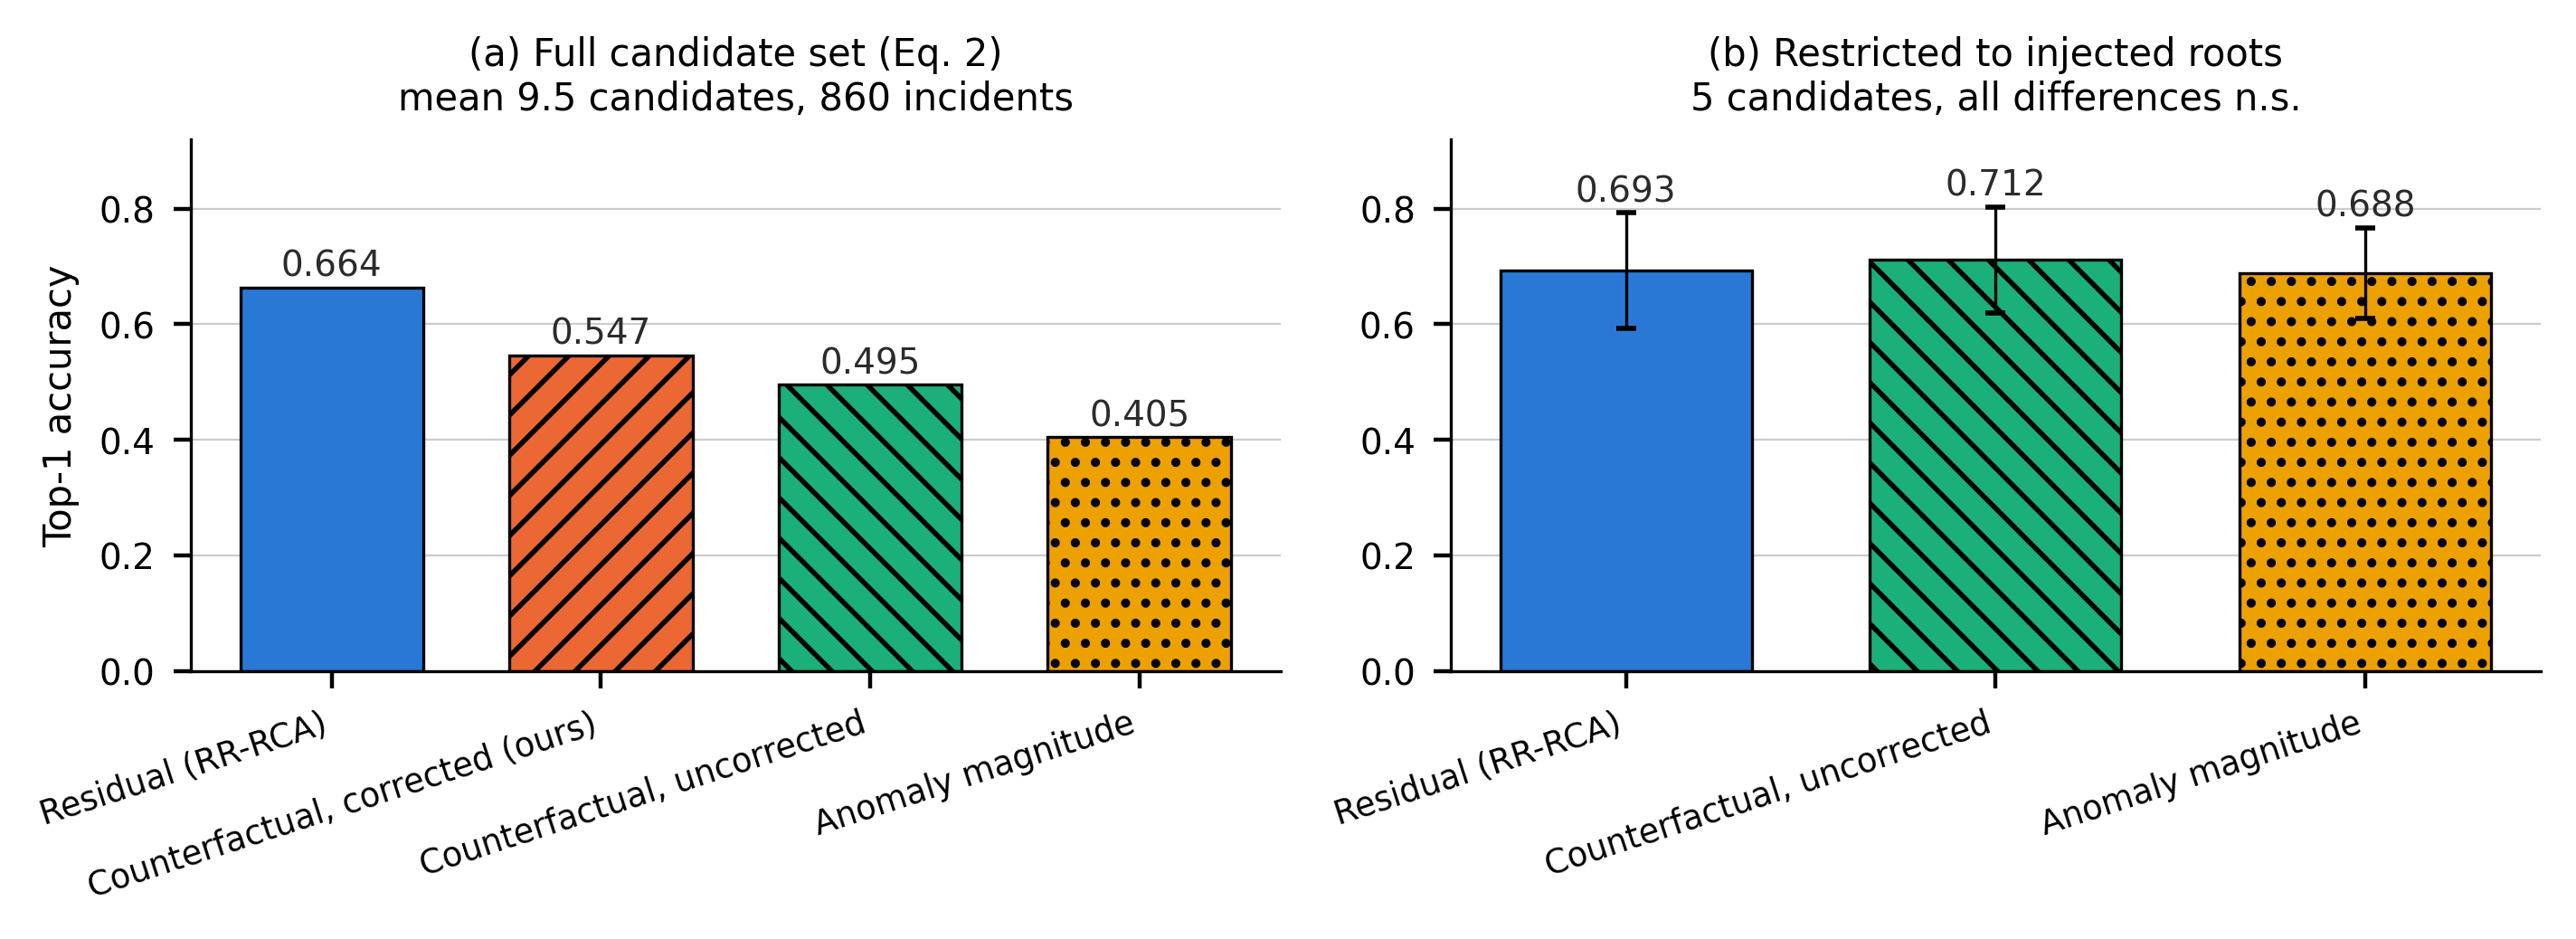
\includegraphics[width=0.95\textwidth]{figure_results_comparison.png}
\caption{Top-1 accuracy of the scoring rules over one architecture-derived DAG. \textbf{(a)} Full candidate set of \eqref{eq:candidate-set}, 860 incidents from 20 seeds. \textbf{(b)} Restricted candidate set of five injected roots; bars are $\pm1$ standard deviation across five seeds, and \emph{n.s.} marks pairs with no significant difference under paired McNemar at $\alpha=0.05$. RR-RCA is our reimplementation of the residual rule of CIRCA \cite{li2022circa}. Hatch patterns keep both panels readable in grayscale.}
\label{fig:results}
\end{figure*}

Fig.~\ref{fig:results} shows the same rules on both candidate sets; the benchmark, not the algorithm, produces the difference between its panels (Section~\ref{sec:results-candset}). Adding the candidate's own deviation to counterfactual scoring is worth $0.051$ Top-1 ($p=9.1\times10^{-9}$; 50 incidents corrected against 6 broken). Both counterfactual variants clear the graph-free floor, so intervention reasoning does contribute something. It simply contributes less than a residual.

\label{sec:results-mechanism}
The aggregate gap comes from one place. Table~\ref{tab:rank} partitions incidents by the rank of the true root among candidates ordered by anomaly magnitude; the intervals are seed-clustered bootstrap percentiles on the paired difference, computed as described in Section~\ref{sec:eval-setup}.

\begin{table}[htbp]
\centering
\caption{Top-1 accuracy by anomaly rank of the true root, 860 incidents.}
\label{tab:rank}
\resizebox{\columnwidth}{!}{%
\begin{tabular}{lccccc}
\toprule
\textbf{Rank of true root} & \textbf{$n$} & \textbf{Ours} & \textbf{Residual} & \textbf{$\Delta$} & \textbf{95\% CI on $\Delta$} \\
\midrule
1 (already loudest) & 348 & 0.486 & \textbf{0.787} & $-0.302$ & $[-0.346, -0.259]$ \\
2--3                & 190 & 0.616 & 0.574 & $+0.042$ & $[-0.038, +0.123]$ \\
4--6                &  92 & 0.380 & 0.446 & $-0.065$ & $[-0.131, +0.011]$ \\
7 or worse          & 230 & 0.648 & 0.639 & $+0.009$ & $[-0.009, +0.026]$ \\
\bottomrule
\end{tabular}%
}
\end{table}

Forty percent of incidents fall in the first row, where anomaly magnitude alone already identifies the root. Residual scoring keeps that answer $0.787$ of the time; counterfactual restoration keeps it only $0.486$ of the time. The counterfactual term overturns correct answers on the easiest incidents, and that single row accounts for most of the aggregate gap.

The reason follows from the structure noted in Section~\ref{sec:method}. Both rules add downstream evidence to the same starting quantity, and both point at the same fact when the graph is right. Residual scoring obtains its evidence from a one-hop observational comparison that mostly agrees with $S_{\mathrm{anom}}$ and rarely overturns it. Counterfactual restoration obtains its evidence by propagating a hypothetical through up to five fitted equations. The difference between the rules is one of scale. Averaged over 210 incidents, the residual term is $0.29$ times the size of the candidate's own deviation, while the counterfactual term is $1.40$ times that size, so the latter dominates $S_{\mathrm{anom}}$ where the former defers to it. The consequence is visible in how often each rule departs from the anomaly ordering: residual scoring does so on $62.9\%$ of incidents and counterfactual restoration on $77.1\%$. Overriding a correct ordering costs accuracy, and it is already correct on the 40\% of incidents in the first row.

The competing explanation can be ruled out. Refitting the baselines and per-edge models on bootstrap resamples of the healthy data, test incidents held fixed, changes the top-1 pick of counterfactual restoration on $4.28\%$ of 4300 incident-refit pairs and of residual scoring on $4.26\%$, and the standard deviation of the top-two margin is if anything lower for counterfactual restoration ($0.030$ against $0.036$). The rules are equally stable under retraining, so sampling noise in the fitted equations is not what separates them.

The remaining rows show no compensating regime, though they differ in how much they establish. Our method is nominally ahead in two of them. On the deeply buried incidents the interval is tight, $[-0.009,+0.026]$, so any advantage either way is at most about two points; that row bounds the difference rather than merely failing to detect one. On the rank 2--3 and rank 4--6 rows the intervals span $0.161$ and $0.142$, wide enough to accommodate a real effect in either direction, so those two rows establish little. The pattern is also not monotone in rank. We tested this partition after observing a coarser one and report it as exploratory. Across five regimes examined in total, gray failures, deep roots, buried roots, this rank partition, and concurrent faults, counterfactual restoration is never significantly ahead.

One alternative explanation can be tested directly. With two simultaneous roots, a downstream metric carries contributions from both cascades, and a regression residual is a joint observational quantity that cannot separate them. Counterfactual restoration simulates $\mathrm{do}(A)$ alone, isolating one root's contribution while leaving the other's cascade intact. This is the one setting in which the two rules ask genuinely different questions rather than the same question with different precision, so it is the setting in which an advantage is most likely to appear if one exists.

We tested it by regenerating with a 40\% concurrent-fault rate and evaluating on the full candidate set. Over 332 multi-fault incidents from 20 seeds, residual scoring reaches Top-1@coverage $0.780$ against $0.654$ for counterfactual restoration and $0.506$ for anomaly magnitude, with a discordant split of 2 to 44 ($p=1.5\times10^{-9}$); Top-2@coverage is $0.840$ against $0.741$ ($p=1.4\times10^{-7}$). The gap barely moves relative to single-fault incidents in the same run ($-0.126$ against $-0.144$), so interventional isolation does not offset a downstream term that overrides the anomaly ordering this often.

Extending that run to 30 seeds and partitioning the 502 multi-fault incidents by how prominent the nearest true root is sharpens the picture. Where the loudest candidate is already a true root, residual scoring leads $0.717$ to $0.545$. Where neither true root is among the three loudest, so that anomaly magnitude is wrong by construction, both causal rules recover a true root on roughly nine incidents in ten ($0.894$ against $0.887$) and disagree on one of 151 incidents. Causal reasoning rescues almost every incident on which the naive signal fails outright; which causal rule performs the rescue does not matter.

Scale alone does not explain everything, because a large term is only harmful when it points the wrong way. If the counterfactual term misdirects when it is propagated through poorly fitted edges, the gap should shrink where those edges fit well and widen where they do not. We split incidents on exactly that: whether every edge leaving the true root reaches $R^2>0.5$ on healthy data. This partition uses ground truth and is an analysis device, not a runtime test.

The prediction holds, and the swing is large. On the 368 incidents whose root has only well-fit out-edges, counterfactual restoration reaches $0.620$ against $0.609$ for residual scoring, a difference of $+0.011$ with a 95\% interval of $[-0.029,+0.054]$. That interval is narrow enough to rule out either rule holding more than a five-point advantage in this regime. On the remaining 492 incidents counterfactual restoration reaches $0.492$ against $0.705$, a difference of $-0.213$ with interval $[-0.252,-0.177]$. Between the two groups counterfactual restoration gains $0.128$ while residual scoring loses $0.096$, so the rules move in opposite directions and the gap closes by $0.224$. This is the pattern Section~\ref{sec:method} predicts.

Two consequences follow. Counterfactual restoration is worth considering when a fabric's structural equations are known to fit well, and not otherwise. The fix is not to prune weak edges from the score: raising the confidence cutoff in \eqref{eq:struct-score} from $0.05$ to as high as $0.7$ leaves accuracy between $0.528$ and $0.550$, because the cutoff drops descendants for every candidate alike. Nor do the rules combine. Letting counterfactual restoration break a close top-two under residual scoring never helps at any gate width, the gentlest gate reaching $0.656$ against $0.664$, and a rank-sum blend behaves the same way. We cannot rule out that a better-designed combination would help, but the simple ones do not.

Table~\ref{tab:regime} reports three further partitions fixed in advance, seven comparisons in all with a Bonferroni factor of seven; negative $\Delta$ favors residual scoring, and intervals are seed-clustered bootstrap percentiles as before. The gap narrows wherever $S_{\mathrm{anom}}$ stops being informative. In those partitions residual scoring falls while counterfactual restoration does not. The intervals separate two kinds of null. On buried roots the difference is bounded within $[-0.037,+0.010]$ on 322 incidents, so whatever advantage either rule holds there is at most about four points. We report a bound rather than equivalence, having specified no margin in advance. On gray failures the interval runs from $-0.150$ to $+0.116$ on only 44 incidents, so that row is consistent with a substantial advantage either way and should not be read as evidence of equivalence.

The finding for RQ1 is therefore that the scoring rules differ, that residual scoring is the most accurate of the four, and that the difference is a matter of how large each rule's downstream term is relative to the candidate's own deviation rather than of what information the two terms carry.

\begin{table}[htbp]
\centering
\caption{Pre-registered partitions, corrected counterfactual restoration against residual scoring, 860 incidents.}
\label{tab:regime}
\resizebox{\columnwidth}{!}{%
\begin{tabular}{lccccc}
\toprule
\textbf{Partition} & \textbf{$n$} & \textbf{Ours} & \textbf{Residual} & \textbf{$\Delta$} & \textbf{95\% CI on $\Delta$} \\
\midrule
All incidents                & 860 & 0.547 & 0.664 & $-0.117$ & $[-0.145, -0.090]$ \\
\midrule
Gray failure                 & 44  & 0.659 & 0.682 & $-0.023$ & $[-0.150, +0.116]$ \\
Normal signal                & 816 & 0.540 & 0.663 & $-0.123$ & $[-0.151, -0.093]$ \\
\midrule
Deep root ($>4$ descendants) & 352 & 0.608 & 0.693 & $-0.085$ & $[-0.122, -0.051]$ \\
Shallow root                 & 508 & 0.504 & 0.644 & $-0.140$ & $[-0.187, -0.093]$ \\
\midrule
Buried root (rank $>3$)      & 322 & 0.571 & 0.584 & $-0.012$ & $[-0.037, +0.010]$ \\
Prominent root (rank $\le3$) & 538 & 0.532 & 0.712 & $-0.180$ & $[-0.225, -0.135]$ \\
\bottomrule
\end{tabular}%
}
\end{table}

\subsection{How Evaluation Design Changes the Answer (RQ2)}
\label{sec:results-candset}
The ordering above disappears if the candidate set is restricted. Table~\ref{tab:candset} repeats the evaluation with $\mathcal{C}$ replaced by the five metrics into which faults are injected, a shortcut common in the RCA literature. All four leading rules become statistically indistinguishable, and anomaly magnitude alone is as good as any of them. Entries are mean $\pm$ standard deviation across the five seeds, and no pairwise difference among the top four is significant.

\begin{table}[htbp]
\centering
\caption{Top-1 accuracy on the restricted candidate set of five injected roots, 5 seeds, 215 incidents.}
\label{tab:candset}
\resizebox{\columnwidth}{!}{%
\begin{tabular}{lcc}
\toprule
\textbf{Scoring rule} & \textbf{Top-1} & \textbf{$p$ vs.\ anomaly magnitude} \\
\midrule
Counterfactual restoration & 0.712 $\pm$ 0.091 & 0.18 \\
Residual scoring (RR-RCA) \cite{li2022circa} & 0.693 $\pm$ 0.100 & 1.00 \\
Anomaly magnitude (no graph) & 0.688 $\pm$ 0.079 & --- \\
Correlation-weighted anomaly & 0.665 $\pm$ 0.060 & 0.58 \\
Distributional divergence \cite{meng2020microcause} & 0.214 $\pm$ 0.009 & $6.0\times10^{-20}$ \\
PageRank centrality & 0.205 $\pm$ 0.009 & $2.3\times10^{-20}$ \\
\bottomrule
\end{tabular}%
}
\end{table}

A single incident shows why. The generator saturates a leaf downlink, so the true root is \texttt{leaf\_link\_util\_downlink} at $S_{\mathrm{anom}}=6.30$. Twelve metrics are anomalous, and six are downstream consequences that look worse than the cause: \texttt{server\_app\_latency} at $8.68$, \texttt{leaf\_queue\_depth} at $8.05$, \texttt{leaf\_buffer\_drops} at $7.92$, and so on. Ranking by anomaly magnitude over the full set picks the application latency and is wrong; both causal rules recover the true root. Restricted to the five injected roots, however, the true root is trivially the loudest, since the next candidate sits at $3.96$ and the rest below $2.63$. Anomaly magnitude is then correct with no causal reasoning at all.

The effect extends to concurrent faults, often presented as the regime that most favors structural reasoning. On multi-fault incidents under the restricted set, counterfactual restoration and anomaly magnitude both reach Top-1@coverage $0.976$ with zero discordant incidents between them ($p=1.0$), while divergence-based ranking reaches $0.366$ ($p=4.2\times10^{-12}$). The gap that looks like evidence for causal propagation is really evidence against divergence scoring.

\label{sec:results-power}
A second evaluation practice inflates effects. Counterfactual refinement applies only to incidents whose two leading candidates are nearly tied, which is $6.6\%$ of fault incidents. At five seeds that subset holds 15 incidents and yields 9 discordant pairs, on which refinement appears to raise Top-1 from $0.250$ to $0.633$. Repeating the identical experiment at forty seeds gives 1720 incidents and 113 ambiguous ones, where the same effect is $0.389$ against $0.460$, a gain of $0.071$ that is not significant ($p=0.27$). The apparent doubling was nine coin flips.

\subsection{Robustness and Fault Realism}
\label{sec:results-secondary}
Table~\ref{tab:secondary} reports both leading rules under telemetry imperfection and under generator configurations matched to measured failure statistics, all on the full candidate set. Residual scoring leads in every condition.

\begin{table}[htbp]
\centering
\caption{Top-1 accuracy under telemetry imperfection and measured fault statistics, full candidate set, 5 seeds.}
\label{tab:secondary}
\resizebox{\columnwidth}{!}{%
\begin{tabular}{lccc}
\toprule
\textbf{Condition} & \textbf{Ours} & \textbf{Residual} & \textbf{$p$} \\
\midrule
Clean                                & 0.553 & 0.684 & $9.7\times10^{-5}$ \\
20\% missing telemetry \cite{little2019statistical} & 0.479 & 0.609 & $2.0\times10^{-5}$ \\
Gaussian noise ($\sigma=0.06$) \cite{scheines2017measurement,zhang2017causal} & 0.409 & 0.553 & $1.8\times10^{-5}$ \\
20\% weakest DAG edges removed \cite{montagna2023assumption,vowels2022d} & 0.581 & 0.688 & $4.3\times10^{-4}$ \\
\midrule
Measured fault prevalence (28.6\%)   & 0.580 & 0.710 & 0.031 \\
Measured class skew                  & 0.470 & 0.605 & $7.3\times10^{-6}$ \\
Prevalence and skew combined         & 0.514 & 0.667 & $1.5\times10^{-3}$ \\
\bottomrule
\end{tabular}%
}
\end{table}

Three observations. Fault prevalence does not matter: moving from a 40\% healthy corpus to the measured 71\% leaves both rules unchanged or slightly better, because ranking happens within an incident and never sees corpus-level balance. Class skew costs both rules roughly $0.08$, so it is a property of the task rather than of either method. And removing the weakest fifth of the DAG edges slightly \emph{improves} counterfactual scoring, from $0.553$ to $0.581$, which is consistent with Section~\ref{sec:results-mechanism}: those edges misdirect multi-hop propagation while contributing little to a one-hop residual.

\subsection{Can the Graph Be Learned? (RQ3)}
\label{sec:results-rq3}
Every result above assumes an architecture-derived graph. Whether that assumption is necessary is an empirical question. Applying shrinkage-regularized partial-correlation discovery \cite{ledoit2004well,hojsgaard2012graphical} to the healthy telemetry of the AIOps Challenge 2020 dataset \cite{netmanaioops2020dataset}, a public corpus of real incidents spanning 40 metrics across application, service and infrastructure layers, recovers a graph with 40 nodes and a single edge, against 28 nodes and 26 edges for the architecture-derived DAG (Fig.~\ref{fig:structural_comparison}). Here AIOps denotes the application of machine learning to IT operations data.

A graph with one edge cannot support multi-hop propagation at all, so none of the rules compared here would be applicable to it. The sparsity persists across the whole threshold sweep, so it is not an artifact of one cut-off. We would not generalize further than that: this is one corpus and one discovery procedure, and a different estimator or a more homogeneous workload could recover more. What it does establish is that on this corpus the learned graph cannot substitute for the architecture-derived one.

\begin{figure}[htbp]
\centering
\resizebox{\columnwidth}{!}{%
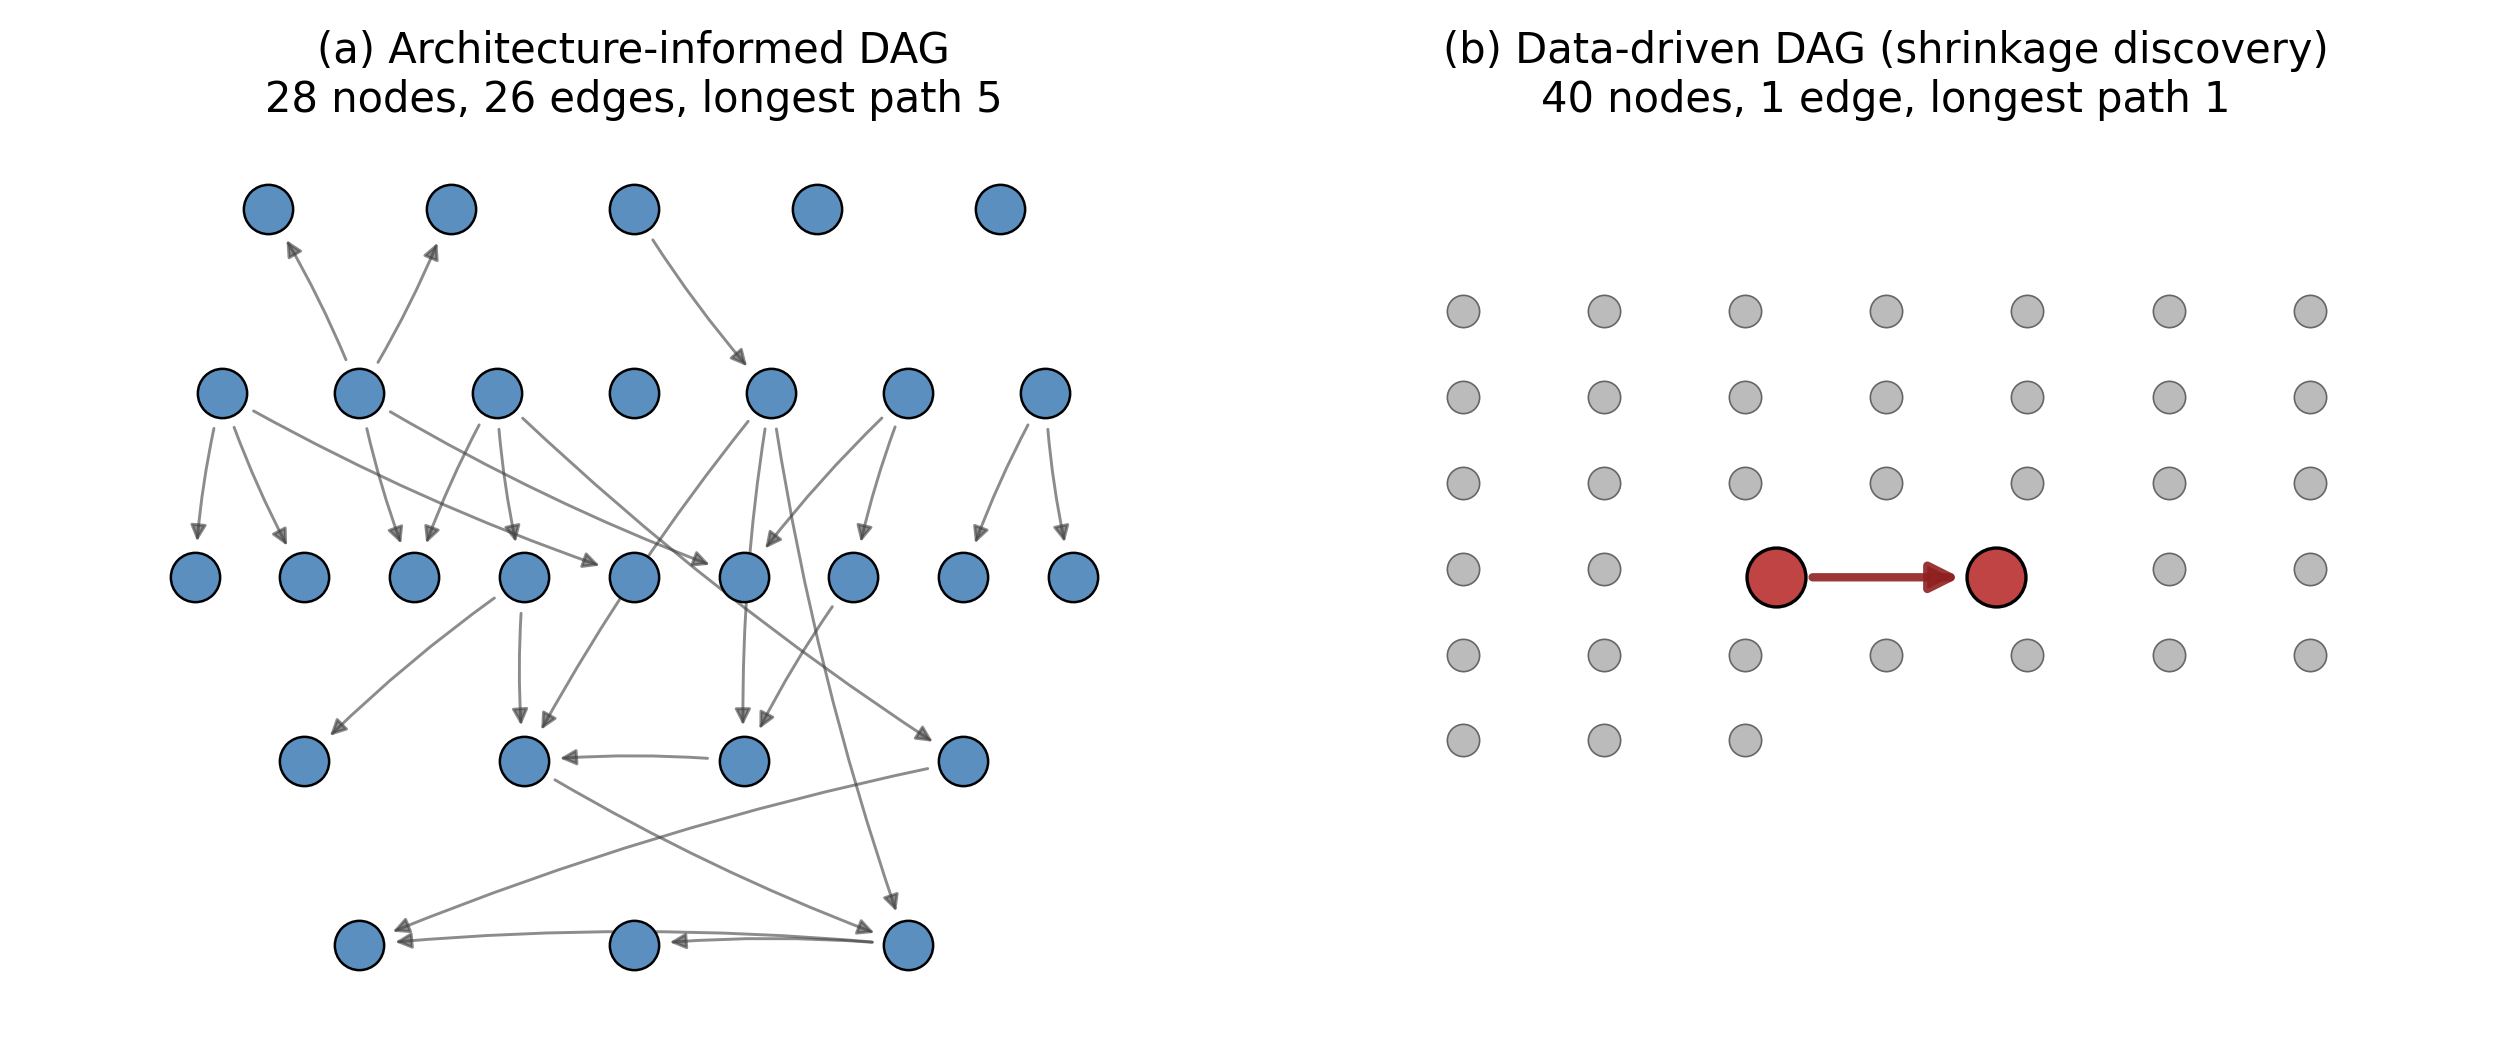
\includegraphics{figure_dag_comparison.png}%
}
\caption{Structural contrast on real telemetry. \textbf{(a)} The architecture-derived DAG (28 nodes, 26 edges, longest path five). \textbf{(b)} The DAG recovered by shrinkage-regularized discovery \cite{ledoit2004well} on AIOps Challenge 2020 healthy telemetry (40 nodes, 1 edge); Arrows denote a directed dependency in each graph; blue nodes in (a) carry at least one such edge, gray nodes in (b) have none, and the two red nodes in (b) are the endpoints of the single recovered edge. The contrast is 26 edges against one.}
\label{fig:structural_comparison}
\end{figure}

\subsection{Cost, Scale and Sensitivity to Settings}
\label{sec:results-cost}
Ranking runs in $0.12$\,ms per incident on the 28-metric graph. To see how that grows, Table~\ref{tab:scaling} times counterfactual restoration, the more expensive of the two leading rules since it propagates through every descendant, on synthetic layered DAGs that preserve the profile of the base graph (five layers, density $0.034$, longest path five) at 28 to 512 nodes. Cost is close to linear in the edge count, which at fixed density grows quadratically with the node count, and reaches $0.66$\,s per incident at 512 metrics and 9{,}000 edges. That is still well inside the 10\,s telemetry cadence, and a production graph derived from architecture is far sparser than the fixed-density extrapolation assumes, so the figures are an upper bound. Residual scoring visits the same descendants without propagating through them, so its cost is of the same order. These figures measure computation on metrics already collected and aligned; collection, not ranking, sets the latency an operator sees.

\begin{table}[htbp]
\centering
\caption{Per-incident ranking latency of counterfactual restoration against graph size.}
\label{tab:scaling}
\begin{tabular}{rrr}
\toprule
\textbf{Nodes} & \textbf{Edges} & \textbf{Latency (ms)} \\
\midrule
 28 &    28 &   $1.1 \pm 0.2$ \\
 64 &   143 &   $8.5 \pm 0.7$ \\
128 &   576 &  $37.6 \pm 2.1$ \\
256 & 2{,}250 & $158.4 \pm 12.0$ \\
512 & 8{,}989 & $656.7 \pm 13.9$ \\
\bottomrule
\end{tabular}
\end{table}

The method has three settings, and the results are not sensitive to any of them in the range tested. The anomaly threshold $\tau=3$ decides membership in the candidate set of \eqref{eq:candidate-set}; the $7.8\%$ of incidents on which the root is not anomalous at $\tau=3$ bound what a higher threshold would cost. The edge-confidence cutoff was swept from $0.05$ to $0.7$ with accuracy moving by at most $0.022$ (Section~\ref{sec:results-mechanism}), and removing the weakest fifth of edges outright moved it by $0.028$ (Table~\ref{tab:secondary}). The partial-correlation threshold of the discovery procedure was swept over four values and the recovered graph never exceeded one edge. The one choice that does matter is the candidate set, which Section~\ref{sec:results-candset} treats as a result rather than a setting.

\section{Discussion and Limitations}
\label{sec:discussion}

\subsection{What the Results Say}
For a practitioner the guidance is simple. Given an architecture-derived graph and healthy-only training, use regression-residual scoring with the candidate's own deviation included. It is the most accurate rule in every condition we tested, and it is cheaper than counterfactual restoration because it makes local comparisons instead of propagating predictions. One exception is worth knowing: where every edge leaving the root fits well, a condition met by 43\% of our incidents, the two rules are indistinguishable and the interval $[-0.029,+0.054]$ bounds any advantage at roughly five points either way. That condition cannot be checked without knowing the answer, so residual scoring remains the default.

For anyone designing an evaluation the guidance is more pointed. Two ordinary-looking choices were enough to reverse or manufacture our conclusions. Restricting candidates to known fault locations made four rules indistinguishable and let a graph-free baseline match a full causal pipeline exactly. Reporting at five seeds produced an effect five times larger than the same experiment at forty. Neither shortcut is exotic, and both appear in work we cite. We would encourage stating the candidate-set definition explicitly and pairing any subgroup claim with the discordant counts behind it.

We also note what did not survive a uniform protocol. Concurrent faults are frequently described as the regime that most favors causal structure. Here they were the regime in which a graph-free baseline tied the full pipeline exactly. Distributional divergence and centrality ranking, by contrast, are worse than everything else by roughly $0.45$ Top-1, so the choice of scoring rule can matter by a wide margin. It does not matter in the direction the recent literature has emphasized.

\subsection{Validating Causal Findings}
Every causal claim above is checked against injected ground truth, which is the strongest validation a synthetic setting allows and one a production setting rarely does. Three checks carry over. First, controlled fault injection on a staging fabric, of the kind chaos-engineering practice already performs, yields labelled incidents on which the rules can be scored as they are here. Second, operator post-incident reviews supply labels for production incidents, at lower volume and with some label noise, and paired tests of the kind used in this paper are well suited to small labelled sets. Third, and specific to intervention scoring, an actual repair is a natural experiment: when the operator fixes the metric the ranker named, the fitted equations predict the order and magnitude in which downstream metrics should recover, and that prediction can be compared with what the telemetry shows. Agreement validates both the graph and the score; disagreement localizes the edge whose equation is wrong. The per-edge fit audit of Section~\ref{sec:method} is the offline form of the same check, and it already predicts where counterfactual restoration can be trusted.

\subsection{Limitations}
\label{sec:limitations}
Training only on healthy telemetry is central to all four rules and constrains them equally. The structural equations describe how metrics move when nothing is wrong, so the model extrapolates when a fault drives metrics far outside their healthy range, which is where a fitted regression is least trustworthy, and a failure mode whose mechanism is absent from healthy operation cannot be represented by this graph at all.

The graph is fixed and hand-derived. We test sensitivity to removing weak edges but do not learn or update structure, and a fabric whose topology changes would need the graph rebuilt. We assume causal sufficiency within the 28 modelled metrics. In the generator that assumption holds by construction: there is no unmeasured variable driving two metrics at once, which is what makes the comparison controlled and is also where it departs most from a production fabric. There, confounding is the rule. Offered load rises and falls with the diurnal cycle and moves link utilization, queue depth and application latency together, and a configuration push or a maintenance window perturbs several devices at once. Each rule is affected, though not identically. Residual scoring fits each edge by regression on healthy data, so a confounder that is absent from the graph biases the fitted coefficient, and the residual at a descendant then partly reflects the confounder rather than the candidate. Counterfactual restoration uses the same coefficients and compounds the bias across every hop it propagates through, which is a further reason its downstream term is the less reliable of the two. The remedy is the standard one, to measure the confounder and add it to the graph as a node; offered load in particular is routinely collected, and we would treat the graph's completeness with respect to such shared drivers as a precondition for deploying either rule.

A deeper limit is that the generator is a statistical model, not a network simulator. It emits metric values from the structural relationships in Fig.~\ref{fig:datacenter_dag} plus noise. It does not simulate packet forwarding, route lookup, queue occupancy under incast or microbursts, buffer drops, or the ECMP hash imbalance that arises from real flow-size distributions. Leaf queue depth and server application latency are coupled as the graph asserts but are not physically produced by the mechanisms those names refer to, and polling jitter and clock skew between collectors are absent. Section~\ref{sec:realism} calibrates prevalence, concurrency and class mix against published measurements, but a generator calibrated to summary statistics is not a production fabric. The comparison establishes the rules' relative behavior under a shared and idealized data-generating process, not their absolute accuracy in deployment, and the account in Section~\ref{sec:results-mechanism} would need re-testing on telemetry whose noise comes from forwarding behavior rather than an additive term.

\section{Conclusion}
We compared four causal scoring rules for root cause analysis in spine-leaf fabrics with the graph, the training regime, the candidate set and the protocol held fixed, so that only the scoring rule varied. On 860 incidents, residual scoring in the style of CIRCA is the most accurate at Top-1 $0.664$, ahead of counterfactual restoration at $0.547$ and anomaly magnitude at $0.405$. The gap has a specific cause: on the 40\% of incidents where the true root is already the most anomalous metric, counterfactual restoration overturns a correct answer more than half the time, because its downstream term is roughly five times larger relative to the candidate's own deviation than the residual term is. The two rules tie where the root's outgoing edges fit well and diverge by $0.211$ where they do not. We also correct a defect in how intervention scoring is usually written: aggregating only downstream effect discards the evidence on the candidate itself, which is worth $0.051$ Top-1 and is a prerequisite for comparing the rules on equal terms.

The findings about evaluation are the ones we would most want carried forward: restricting the candidate set to known fault locations makes all four rules statistically indistinguishable and lets a graph-free baseline match a full causal pipeline exactly, and five seeds report an effect five times larger than forty. Data-driven discovery on real telemetry recovered one edge across forty metrics, so on that corpus the architecture was the only workable source of the graph. Two next steps follow: a combination of the two rules that reconciles their terms on a common scale, since gating and rank-sum blending both failed, and a repeat of this comparison on a fabric emulator whose telemetry comes from forwarding behavior rather than fitted equations.

\section*{Data and Code Availability}
The generator, the 26-edge DAG, all four scoring rules, every evaluation script behind the tables and figures, the result files they were typeset from, and the figure generators are available at \url{https://github.com/navinsuvarna786/controlled-causal-rca}. The AIOps Challenge 2020 telemetry is publicly distributed \cite{netmanaioops2020dataset}.

\bibliographystyle{IEEEtran}
\bibliography{references}

\end{document}
